\documentclass[a4paper, 12pt]{article}
\usepackage{cmap}
\usepackage[utf8]{inputenc}
\usepackage[english, russian]{babel}
\usepackage[left=2cm, right=2cm, top=2cm, bottom=2cm]{geometry}
\usepackage{amsfonts,amssymb}
\usepackage{amsmath}
\usepackage{amsthm}
\usepackage{titlesec}
\usepackage{graphicx}
\usepackage{mathtools}
\usepackage{hyperref}

 \newcommand{\tit}[1]{\begin{center}{\bf{\Large #1}}\end{center}}
 \newcommand{\aut}[1]{\centerline{{\bf #1}}}
 \newcommand{\cityorg}[1]{\centerline{\it #1}}
 \newcommand{\email}[1]{\centerline{{\small e-mail: #1}}\vspace{\baselineskip}}
\providecommand{\keywords}[1]{\textbf{\textit{Ключевые слова:}} #1}
\newcommand{\norm}[1]{\left\lVert#1\right\rVert}
\newcommand{\normb}[1]{\left\lVert\textbf{#1}\right\rVert}

\begin{document}

\sloppy
 \tit{Цилиндрическая маскировка при помощи оптимизированных конечных 
 многослойных параметров для наклонного падения}
 \aut{Baile Zhang and Bae-Ian Wu}

\begin{abstract}
Мы предлагаем многослойную цилиндрическую маскировочную оболочку, 
оптимизированную для непрямого падения путем комбинации аналитического 
формализма и применении генетических алгоритмов. 
Мы покажем, что используя только четыре однородных, анизотропных слоя с 
параметрами, не принимающими больших 
значений, рассеяние для падения под непрямым углом может быть уменьшено на 
два порядка. Несмотря на то, что оптимизация применялась для одного угла 
падения, оболочка показывает уменьшение рассеяния для широкого диапазона углов.
\end{abstract}

В последнее время было приложено много усилий для проектирования и воплощения 
метаматериальных маскирующих оболочек используя трансформационные методы 
\cite{1}-\cite{9}.
Было доказано, что совершенная маскирующая оболочка, созданная путем 
трансформации пустого электромагнитного пространства \cite{1}, может идеально 
скрывать произвольный объект \cite{5}-\cite{7}, в то время как единственный 
электромагнитный механизм, способный обнаружить
совершенную оболочку в пределах ее рабочего диапазона, требует экстремальных 
условий \cite{10}. Однако, на текущий момент практическая разработка 
метаматериальной маскирующей оболочки еще далека от практической реализации в 
силу того, что строгие требования идеальной оболочки, такие как непрерывно
изменяющиеся параметры, которые приближаются к экстремальным значениям в 
некоторых областях, представляют трудность для практического изготовления. 
Хотя выполненная перед этим упрощенная цилиндрическая оболочка \cite{3}
может умеренно снижать рассеяние, по своей сути она все еще видна \cite{11} и 
работает только для падения под прямым углом в двумерном случае. Недавно были 
высказаны теоретические предположения по преодолению недостатков
непрерывных и экcтремальных параметров путем оптимизации структуры, состоящей 
из малого количества однородных и анизотропных метаматериалов, для построения 
практической оболочки \cite{12, 13}. Однако, также как и в предыдущих 
исследованиях, рассматривалось только падение под прямым углом и, 
следовательно, результаты работают только в двумерной геометрии. Расширение 
двумерного дизайна до трехмерного станет еще одним шагом до практически 
используемой реализации маскирующих покрытий.

В этой работе мы представляем маскирующую оболочку, построенную при помощи 
только четырех слоев метаматериалов, которая может работать для широкого 
диапазона падающих углов. Наша работа может быть
интерпретирована как расширение и дополнение чисто двумерных моделей до более 
физичных и практических трехмерных моделей \cite{12, 13}. Мы используем 
генетическую оптимизацию для глобального поиска оптимизированного 
набора параметров. Оптимизация многослойной оболочки выполнена для угла 
падения равного 30$^{\circ}$. Наш метод может быть использован как инструкция 
для будущих реализаций метаматериальных маскирующих оболочек.

\begin{figure}
  \centering
  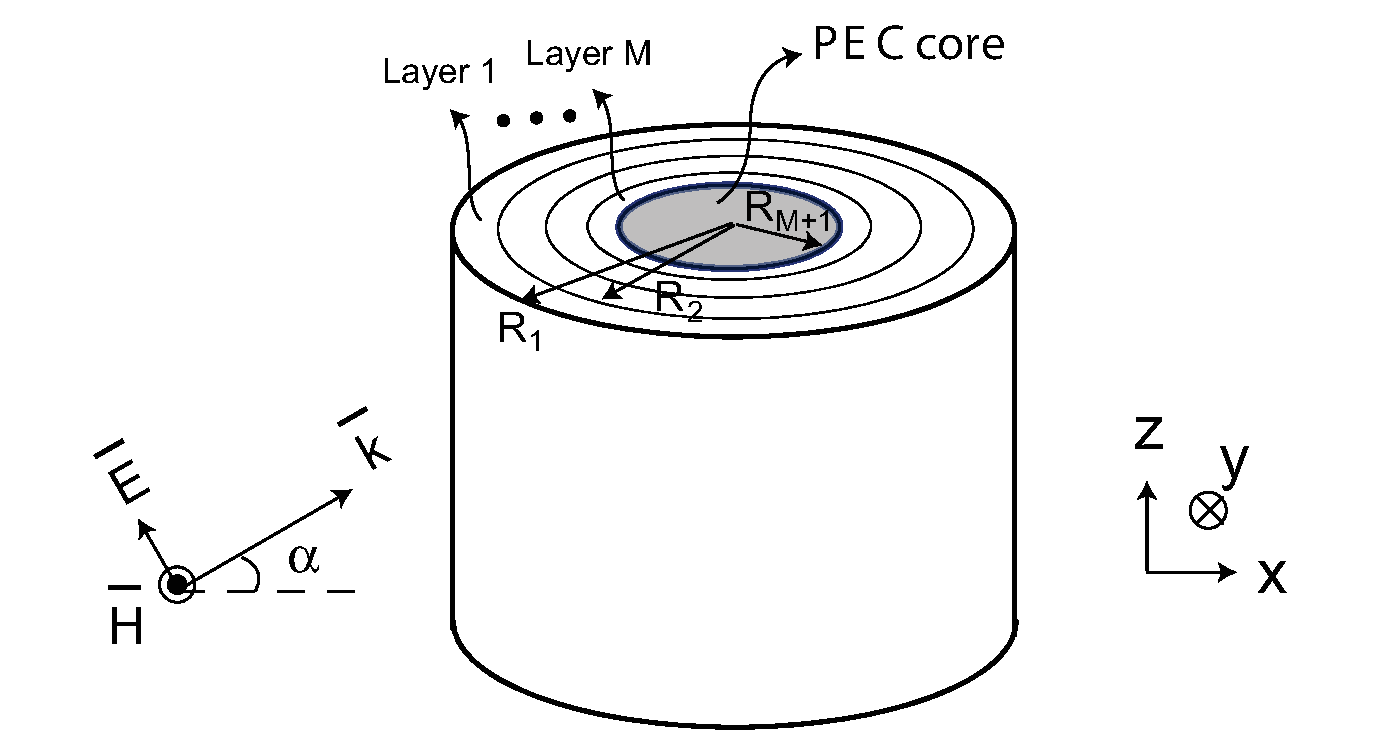
\includegraphics[width=0.5\columnwidth,draft=false]{Fig_1}
  \caption{
  Конфигурация четырехслойной оболочки, когда вертикально поляризованная волна падает под углом $\alpha$.
  }
  \label{fig:model}
\end{figure}

Геометрия модели многослойной цилиндрической маскирующей оболочки показана на 
Рис. \ref{fig:model}, где идеальный электрический проводник (PEC) 
цилиндрической формы, радиуса $R_{M+1}$ покрывается многослойной 
цилиндрической оболочкой с внутренним радиусом $R_{M+1}$ и 
внешним радиусом $R_1$. Между $R_1$ и $R_{M+1}$ расположены $M$ слоев, 
обозначенные $m (1 \le m \le M)$ с различными радиусами, варьирующимся от $R_1$
до $R_M$. Существенные параметры каждого слоя 
($\epsilon_\rho$, $\epsilon_\phi$, $\epsilon_z$, $\mu_\rho$, 
$\mu_\phi$ и $\mu_z$) предполагаются однородными. 
В области $r > R_1$ находится свободное пространство. Падающая 
электромагнитная волна падает на многослойную цилиндрическую оболочку под 
углом $\alpha$ по отношению к оси $xy$. Без потери общности, мы рассматриваем
вертикальную поляризацию, как показано на Рис.~\ref{fig:model}. Следовательно, 
единичная волна принимает вид 
$\overline{E}_i =(-\hat x\sin \alpha + \hat z \cos \alpha) 
e^{ikz \sin \alpha + ikx\cos \alpha}$.

Для падения под непрямым углом сложность заключается в том, что для волнового 
уравнение внутри каждого слоя не найдено аналитическое решение. Мы предоставили
метод для вычисления рассеяния от общей цилиндрической оболочки при непрямом
падении \cite{14}, основанный на методе переменных состояния \cite{15}.
Мы применяем этот метод в каждом слое для расчета матрицы распространения для
каждого соответствующего состояния, соответственно. Их произведения будет 
финальным состоянием матрицы распространения всей многослойной структуры.
Если мы разделим каждый слой на $N$ подслоев $N \gg 1$, уравнение
распространения состояния будет иметь вид
\begin{eqnarray}
&\overline V (R_{M+1}) = \nonumber & \\
&\left[ \prod_{j=(M-1)N+1}^{MN}(\overline{\overline I} + \Delta \rho
\overline{\overline T}(\rho_{j})) \right]
 \nonumber \cdot \left[ \prod_{j=(M-2)N+1}^{(M-1)N}(\overline{\overline I} +
\Delta \rho \overline{\overline T}(\rho_{j})) \right]&\nonumber
\\
&\cdot \cdot \cdot & \nonumber
\\
 & \cdot \left[
\prod_{j=1}^{N}(\overline{\overline I} + \Delta \rho
\overline{\overline T}(\rho_{j})) \right] 
 \cdot \overline V (R_1)6&
\end{eqnarray}
где четырех-размерный вектор 
$\overline V = [E_z ~E_\phi ~H_z~H_\phi]^T$ ~--- вектор состояния. 
После получения матрицы распространения, мы можем найти распределения поля
во всем пространстве \cite{14}. 
Теперь, путем применения генетической оптимизации,
получим многослойную оболочку, применяемую для непрямого падения.

\begin{figure}
  \centering
  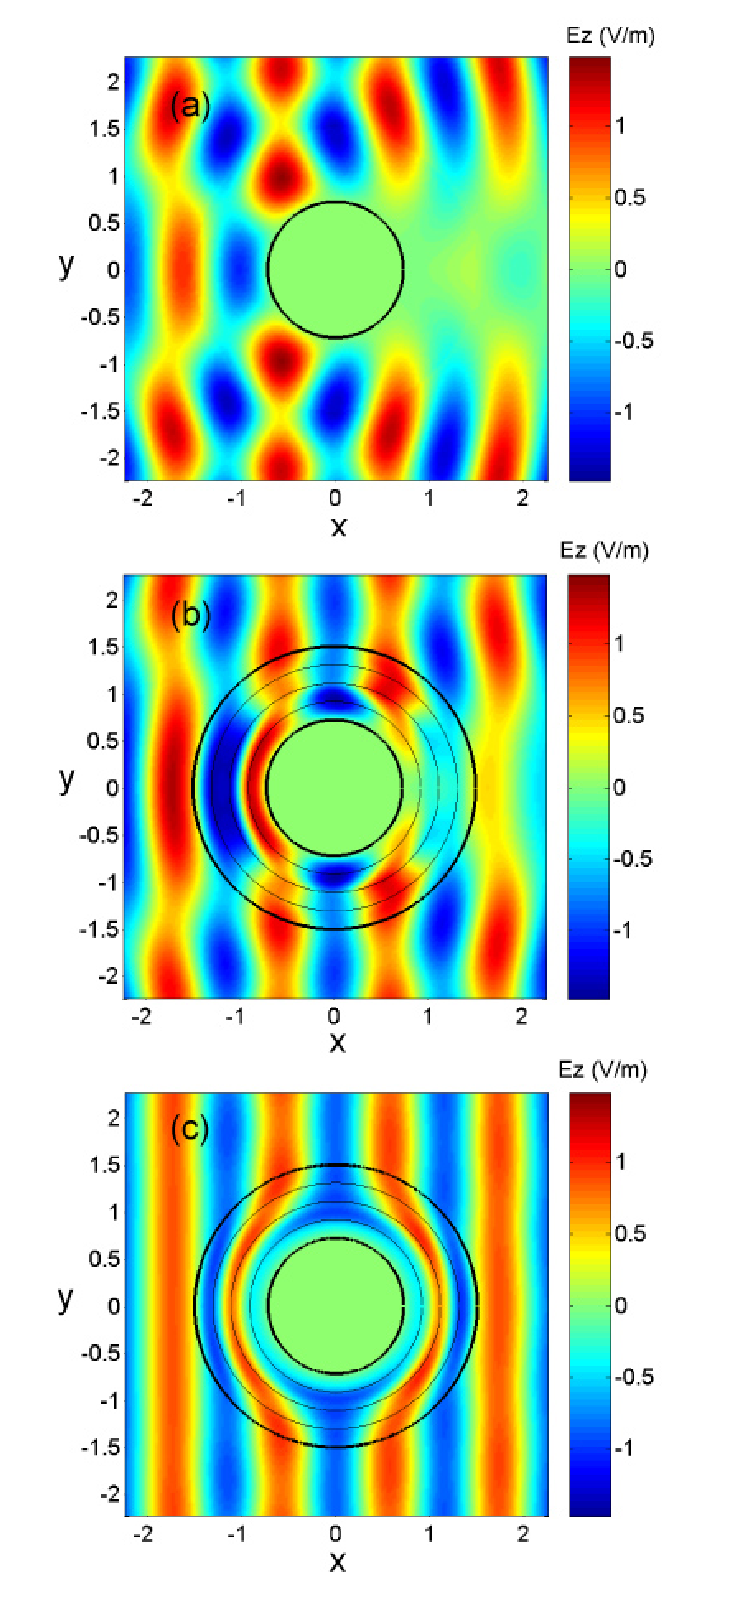
\includegraphics[width=0.5\columnwidth,draft=false]{Fig_2}
  \caption{
  Распределение поля $E_z$ в плоскости $xy$ при рассеянии от (a) непокрытого
  PEC цилиндра, (b) четырехслойной с тремя оптимизированными параметрами 
  $(\epsilon_z, \mu_\rho$ и $\mu_\phi)$, и (c) четырехслойнойная оболочка
  с шестью оптимизированными параметрами, когда вертикально поляризованная плоская волна падает под непрямым углом $30^{\circ}$ слева на право.
  От (a) до (c) эффективность рассеяния $Q_{sca}$ равна 
  1.175, 0.498 и 0.013 соответственно. }
  \label{fig:field}
\end{figure}

Для сравнения с производительностью упрощенной оболочки при непрямом падении,
рассмотрена цилиндрическая структура с такими же размерами, как в \cite{14},
то есть $R_1 = 1.5\lambda_0=2.08R_{M+1}$. Мы задали количество слоев $M$ 
равное четырем, при этом все слои имеют одинаковую толщину. Так же нами было
поставлено другое условие, заключающееся в том, что все существенные параметры
должны быть меньше 10. Угол падения выбран равным $\alpha = 30^\circ$.
В генетическом алгоритме эффективность рассеяния в дальней зоне $Q_{sca}$ 
\cite{7} или же сечение рассеяния, нормализованное на единичное геометрическое 
сечение $2R_{M+1}$, выбирается как функция для минимизации.

Сначала мы рисуем рассеяние с непокрытого PEC ядра радиуса $0.712\lambda_0$
как указано в ссылке, поле $E_z$ в плоскости $xy$ изображено на 
Рис.~\ref{fig:field}(a). Показано, что рассеяние достаточно велико, а 
эффективность рассеяния в этом случае равно 1.175. Отметим, что хотя 
падающая волна строго вертикально поляризована, отраженная волна в общем
случае состоит из обеих вертикальной и горизонтальной поляризации, где
только у вертикальной поляризации имеется компонента $E_z$. Следующее задание 
заключается в минимизации $Q_{sca}$ путем оптимизации.

У нас имеются два метода оптимизации. Один заключается в управлении 
$\epsilon_z, \mu_\rho$ и $\mu_\phi$ в каждом слое (предыдущая упрощенная
оболочка для падения под прямым углом \cite{3} нуждалась только в этих трех 
параметрах), полагая $\epsilon_\rho, \epsilon_\phi$ и $\mu_z$ константами,
равными 1. Другой метод состоит в управлении всеми шестью существенными 
параметрами в каждом слое. Производительность этих двух оптимизированных
четырехслойных оболочек показана на Рис.~\ref{fig:field}(b) и 
Рис.~\ref{fig:field}(c). Их относительные существенные параметры приведены
в Таблице~\ref{table:params}. На Рис.~\ref{fig:field}(b) можно увидеть,
что при управлении только тремя параметрами в каждом слое можно сильно
умееньшеить общее рассеяние по сравнению с непокрытым PEC ядром на 
Рис.~\ref{fig:field}(a). Эффективность рассеяния $Q_{sca}$ 
уменьшается с 1.175 до 0.498. После оптимизации всех шести слоев в каждом слое
эффективность рассеяния $Q_{sca}$ становится равной $0.013$, что близко
к "идеальной невидимости"\, как показано на Рис.~\ref{fig:field}(с).
Стоит отметить, что несмотря на то, что четырехслойная оболочка на 
Рис.~\ref{fig:field}(с) получена оптимизацией при одном угле падения 
$30^\circ$, она продолжает работать для других углов. На Рис.~\ref{fig:sca}
мы можем видеть, что эта оболочка показывает удовлетворительные результаты для
широкого диапазона углов падения, даже когда некоторые тангенциальные потери
входят во все существенные параметры оболочки.

\begin{table}
\begin{center}
\begin{tabular}{|c|ccc|ccc|}
\hline
 I&\multicolumn{6}{c|}{Оптимизация трех парамеров} \\
\hline
 Слой & $\mu_{\rho}$ & $\mu_{\phi}$ & $\epsilon_{z}$  & $\epsilon_{\rho}$ & $\epsilon_{\phi}$ & $\mu_{z}$ \\
\hline
1 & 0.962 & 1.423 & 1.154 & 1 & 1 & 1\\
 2 & 1.128 &0.160  &  0.598 & 1 & 1 & 1\\
 3 & 0.792 & 2.754 & 1.321 &1 &  1 & 1\\
 4 & 0.665 & 1.025 & 2.625 &1 &  1 & 1 \\
 \hline
  II&\multicolumn{6}{c|}{Оптимизация шести параметров} \\
\hline
 Слой & $\mu_{\rho}$ & $\mu_{\phi}$ & $\epsilon_{z}$  & $\epsilon_{\rho}$ & $\epsilon_{\phi}$ & $\mu_{z}$ \\
\hline
1 & 0.550 & 2.320 & 1.725 & 0.438 & 1.781 & 3.409\\
 2 & 0.283 & 3.584 & 1.657 &  0.262 & 3.953 & 0.037\\
 3 & 0.224 & 8.204 & 0.614& 0.189 & 8.674 & 1.754\\
 4 & 0.057 & 9.994 & 0.015 & 1.540 & 9.069 & 0.030 \\
\hline
\end{tabular}
\caption{\label{table:params} Относительные существенные параметры для
оптимизированных четырехслойных оболочек путем (I) оптимизации трех
параметров в каждом слое и (II) оптимизации шести параметров в каждом слое.}
\end{center}
\end{table}

В принципе, мы можем приписать этот феномен низкого рассеяния к
деструктивной интерференции между волнами от первого отражения самой внешней
границы и всеми переданными волнами (waves from the total transmission) 
изнутри оболочки наружу \cite{12}. 
Однако, сценарий непрямого падения более сложен,
чем случай нормального падения, так как обе поляризации должны быть 
оптимизированы одновременно. Для случая нормального падения, так как 
вертикально поляризованные волны и горизонтально поляризованные волны 
разделены, отражение и трансмиссия на отдельных границах между сопряженными
слоями затронет одну поляризацию без влияния от другой поляризации. 
Следовательно, относительно легче достичь деструктивной интерференции
вне оболочки. Когда угол падения отличен от нуля, вертикально и горизонтально
поляризованные волны становятся связанными. Таким образом, возникает
необходимость в большем количестве степеней свободы, чтобы при оптимизации
структуры достигнуть деструктивной интерференции для обеих поляризаций.
Это объясняет гораздо лучшую производительность для четырехслойной оболочки
при оптимизации всех ее существенных параметров в каждом слое 
[Рис.~\ref{fig:field}(с)], в противовес всего лишь трем параметром
Рис.~\ref{fig:field}(b).

\begin{figure}
\centering
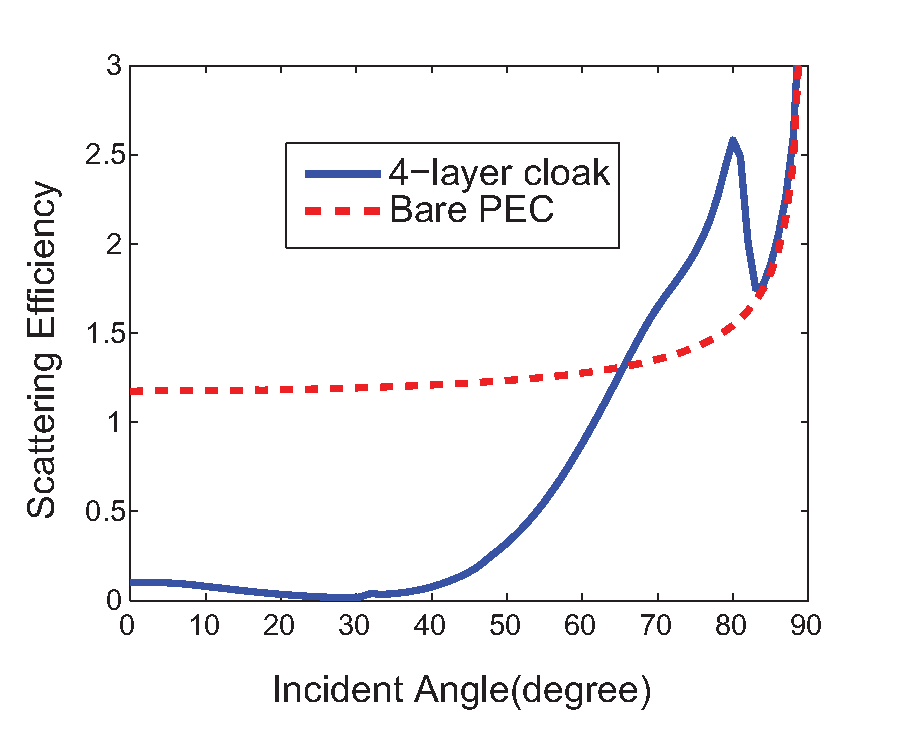
\includegraphics[width=0.5\columnwidth,draft=false]{Fig_3}
\caption{\label{fig:sca} Зависимость эффективности рассеяния $Q_{sca}$ 
от угла падения для четрехслойной оболочки, достигнутая при оптимизации
всех шести параметромметров в каждом слое оболочки. Пунктирные кривые обозначают
эффективности рассеяния от оболочки с тангенциальными потерями 0.05 и 0.1, и
от непокрытого PEC ядра без оболочки, соответственно.}
\end{figure}

В заключение, мы предложили метод получения работающей для непрямого падения
многослойной цилиндрической оболочки путем комбинации аналитического алгоритма 
для трехмерного рассеяния и генетической оптимизации. Мы показали, что
используя только четыре слоя, состоящих из однородных и анизотропных
материалов, с существенными параметрами принимающими конечные значения,
рассеяния от оболочки при непрямом падении может быть уменьшено на два порядка.
Хотя оптимизация выполнялась для одного угла падения, производительность
оболочки оказалась удовлетворительной для широкого диапазона углов падения.
Эта работа является расширением и дополнением предыдущих двумерных моделей
[12, 13] в трехмерной аналогии. Мы предвидим, что комбинация аналитического 
алгоритма трехмерного рассеяния и генетической оптимизация является мощным
инструментом, который будет использован в большом количестве подходов
к практической реализации трехмерных маскирующих оболочек в будущем.

\begin{thebibliography}{99}

\bibitem{1} J. B. Pendry, D. Schurig, and D.R. Smith,  ``Controlling Electromagnetic Fields,'' Science {\bf 312,} 1780 (2006).

\bibitem{2} U. Leonhardt, Science, ``Optical Conformal Mapping,''  {\bf 312,} 1777 (2006).

\bibitem{3} D. Schurig, J.~J. Mock, B.~J. Justice, S.~A. Cummer, J.~B. Pendry, A.~F. Starr, and D.~R. Smith, ``Metamaterial Electromagnetic Cloak at Microwave Frequencies,'' Science {\bf 314,}
977 (2006).

\bibitem {4} S.~A. Cummer, B.~I. Popa, D. Schurig, D.~R. Smith, and J.~B. Pendry, ``Full-wave Simulations of Electromagnetic Cloaking Structures,'' Phys. Rev. E, {\bf 74,} 036621 (2006).

\bibitem{5} H. Chen, B.~I. Wu, B. Zhang, and J.~A. Kong, ``Electromagnetic Wave Interactions with a Metamaterial Cloak,'' Phys. Rev. Lett. {\bf 99,} 063903 (2007).

\bibitem {6} Z. Ruan, M. Yan, C.~W. Neff, and M. Qiu, ``Ideal Cylindrical Cloak: Perfect but Sensitive to Tiny Perturbations,'' Phys. Rev. Lett. {\bf 99}, 113903 (2007).

\bibitem {7} B. Zhang, H. Chen, B.-I. Wu, Y. Luo, L. Ran, and J.~A. Kong, ``Response of a Cylindrical Invisibility Cloak to Electromagnetic Waves,'' Phys. Rev. B {\bf 76}, 121101(R) ( 2007).

\bibitem {8} W. Cai, U.~K. Chettiar, A.~V. Kildishev, and V.~M. Shalaev, ``Optical Cloaking with Metamaterials,'' Nat. Photonics {\bf 1}, 224 (2007).

\bibitem {9} Y. Huang, Y. Feng, and T. Jiang, ``Electromagnetic Cloaking by Layered Structure of
Homogeneous Isotropic Materials,'' Opt. Express {\bf 15}, 11133
(2007).

\bibitem {10} B. Zhang, and B.-I. Wu, 
``Electromagnetic Detection of a Perfect Invisibility Cloak,''  {\bf 103}, 243901
(2009).

\bibitem {11} M. Yan, Z. Ruan, and M. Qiu, ``Cylindrical Invisibility Cloak with Simplified Material Parameters is Inherently Visible,''  {\bf 99} 233901 (2007).


\bibitem {12} S. Xi, H. Chen, B. Zhang, B.-I. Wu, and J.~A. Kong, ``Route to Low-scattering Cylindrical Cloaks with Finite Permittivity and Permeability,'' Phys. Rev. B {\bf 79}, 155122 (2009).

\bibitem {13} B.-I. Popa, and S.~A. Cummer, ``Cloaking with Optimized Homogeneous Anisotropic Layers,''  Phys. Rev. A {\bf 79}, 023806 (2009).


\bibitem {14} B. Zhang, H. Chen, and B.-I. Wu, ``Limitations of High-order
Transformation and Incident Angle on Simplified Invisibility
Cloaks,'' Opt. Express {\bf 16}, 14655 (2008).

\bibitem {15} W.~C. Chew, Waves and Fields in Inhomogeneous Meida,  IEEE Press (1995).





\end{thebibliography}
\end{document}